%\documentclass[sigconf,natbib=false]{acmart}
\documentclass{scrartcl}
%\documentclass{article}
%%%%%%%%
% Packages
%%%%%%%%

\usepackage[backend=bibtex]{biblatex}

% Filter warnings issued by package biblatex starting with "Patching footnotes failed"
% Source: https://tex.stackexchange.com/questions/202988/beamer-patching-footnotes-warning-patching-footnotes-failed-footnote-detectio
\usepackage{silence}
\WarningFilter{biblatex}{Patching footnotes failed}

% For formal tables
\usepackage{booktabs} 
\usepackage{hyperref}
\usepackage{cleveref}

\usepackage{csquotes}

%%%%%%%%
% Remove copyright
%%%%%%%%
%\setcopyright{none}
%\settopmatter{printacmref=false}
%\acmISBN{} % set this to remove ISBN
%\acmDOI{} % set this to remove DOI

\newcommand{\burl}[1]{\textbf{\url{#1}}}

%%%%%%%%
% Meta information
%%%%%%%%
%\acmConference[]
%	{Masterpraktikum Lehrstuhl X}
%	{SoSe \the\year}


%%%%%%%%
% Bibliography sources
%%%%%%%%

% * you can use a remote bibliography from BibSonomy (change 'dmir' to your own username)
%\addbibresource[location=remote]{http://www.bibsonomy.org/bib/user/dmir/myown}

% * or a local file
\addbibresource{bibliography.bib}



\begin{document}

%%%%%%%%
% Front matter
%%%%%%%%

\title{Bericht Masterpraktikum}
%\subtitle{Lehrstuhl X, }

\author{Armin Bernstetter (Matrikelnr. 1876874)}
%\affiliation{%
%  \institution{University of W\"urzburg}
%  \today
%}
% \email{trovato@corporation.com}

\maketitle

\begin{abstract}
\textbf{GER}
Basis für das Projekt dieses Masterpraktikums war die grundlegende Idee, GPT-2 für einen deutschen Textkorpus zu adaptieren. Dazu wurde zunächst ein bereits bestehender Korpus erweitert mit Texten eines deutschsprachigen Internetforums. Anschließend wurden auf diesem erweiterten Korpus language models trainiert (ELMo und GPT-2). Der durch das größte dieser GPT-2 Modelle generierte deutsche Text ist von annähernd natürlichsprachlicher Qualität und eignet sich als \enquote{proof of concept}.
\\\\
\textbf{ENG}
This project was based on the idea of applying GPT-2 to a german web text corpus. For this, an existing corpus was extended with text from a german internet forum. This data set was then used to train language models (ELMo and GPT-2). The largest of these GPT-2 models generates rather high-quality german text and serves as a proof of concept justifying further work.
\end{abstract}


%%%%%%%%
% Content
%%%%%%%%



\section{Introduction/Motivation}

The general task of this project was to expand a corpus of german text and then train language models on this corpus.

This was based on the overwhelming success of OpenAI's \footnote{\url{https://openai.com/}} GPT-2 project \cite{radford2019language} which trained a language model on 40GB of english web text. The model was so successful in tasks such as text generation that OpenAI refused to release the training code, the full training data and the entire model out of ethical reasons. The concern was that malicious parties could use GPT-2 to generate e.g. fake news for their own good and to spread misinformation.

Therefore it was necessary to create a new dataset, train the models on this corpus and check whether GPT-2 also works for text in languages other than English, e.g. German.


\section{Crawler}

Several available german text corpora were already included in the existing corpus. This included the german Wikipedia and novels. 
To extend the corpus, the plan was to crawl several german webpages for useful text data.

\paragraph{Reddit}
Pages that were considered initially were german subreddits on Reddit. Reddit is a social media site for sharing and discussing content. It is organized into so called subreddits which are boards mostly focussed on single topics. Relevant for this project were subreddits such as \textit{/r/de}\footnote{\url{https://www.reddit.com/r/de}}, the main german-language subreddit or \textit{/r/de\_iama}\footnote{\url{https://www.reddit.com/r/de\_iama}}, probably the german subreddit with the most subscribed users (around 330.000 as of 2019-09-30).

Reddit's API unfortunately limits the amount of requests a script can make and would require actively trying to avoid this limitation.

For future work it could make sense to look into \url{https://pushshift.io/} which offers a number of Reddit data dumps, mostly from some years ago.

\paragraph{Wattpad}

Another page that was considered briefly was Wattpad \footnote{\url{https://www.wattpad.com/}}, a \enquote{social storytelling} platform. Users can share their own stories there and read those of other users. Upon examination of the web page's structure and HTML code it was decided that Wattpad obviously are not keen on users crawling their site. Therefore Wattpad was dismissed as well.

\paragraph{Team-Andro} The website Team-Andro \footnote{\url{https://www.team-andro.com/}} is a german Fitness and Bodybuilding board. It contains articles on training, nutrition, sport events and more. More importantly, however, it is accompanied by a large german web forum with a user count of almost 300.000 and around 10 million forum posts in total (last checked 2019-09-25).

Upon inquiry the site administrator provided some helpful advice and a link to Team-Andro's sitemap. Unfortunately they had to decline the request for a simple and complete database dump of the forum's posts. Due to the forum's database structure it would not have been easily possible to exclude e.g. internal posts by administrators that need to remain private.

The forum uses the standard \textit{phpBB3}\footnote{\url{https://www.phpbb.com/}} board software and therefore the crawler should be applicable for other \textit{phpBB} boards with minor adaptations.


Using the sitemap, it was possible to simply iterate through most of the forum's publicly available HTML pages. Team-Andro's sitemap contains around 80 sub-sitemaps each containing links to around 10.000 forum topics/pages. These pages were then parsed from HTML and saved in a directory structure representing the forum structure of Team-Andro with each post represented as one text file. Additionally, meta data such as user names, time stamps etc were saved in a mongoDB database.
Each of the forum topics contains at least one text post by a user and the largest topic on the entire site contains around 700.000 posts.


\section{The Dataset}

Prior to the addition of the Team-Andro text data, the existing corpus consisted of a collection of various german text sources. This corpus contains for example the german Wikipedia and german novels and amounted to around 7.7GB of plain text files in total.


The Team-Andro corpus consists of mostly german web text. As such it is often unstructured, meaningless text without contiguous sentences. It is not as \enquote{bad} as e.g. text data from Twitch chat but still contains its fair share of internet slang and site-internal phrases and memes. Despite having a large Off-Topic subforum, a lot of the text is still focussed on topics such as sports in general and fitness/bodybuilding/weightlifting in particular.

The text also contains some special cases due to the forum software.
For example one of the phrases which are extremely overrepresented in the corpus is \enquote{\textit{[username] hat am [date] geschrieben:}}.
This indicates a quote of an earlier post inside a new post which often results in repetitions and nested posts of multiple levels.

In addition to a corpus with a directory structure representing the forum structure, the Team-Andro text was also merged into simple text files with 50MB each. This corpus consists of 2.8GB of plain text files.

The combined corpus used in this project therefore had around 10.5GB of text with 75\% used as training data and 25\% set aside as \enquote{heldout}.

For minor experiments, a \enquote{minimal corpus} was created consisting only of one 50MB file from the existing corpus and Team-Andro each.



\section{ELMo}

ELMo is a deep contextualized word representation \cite{Peters:2018}. A tensorflow implementation of a deep bidirectional language model used to train ELMo representations is available on github \footnote{\url{https://github.com/allenai/bilm-tf}}.

This implementation was used in this project to ease into the topic of training language models. A model was trained on the entire training data (75\% of the overall corpus) for around 2 weeks and 1.877.500 steps.

The trained model was successfully used to output word embeddings. Further examination of the trained model as well as tasks such as text generation have not been undertaken.


\section{GPT-2}
GPT-2 is a language model trained by OpenAI on a large corpus of web text \cite{radford2019language}.

OpenAI refrained from publicizing their training code and larger versions of pretrained models.
Github user \enquote{nshepperd} created a fork of GPT-2 containing Python scripts to train a GPT-2 model. This code was successfully used by blogger and author \enquote{Gwern} (\url{https://www.gwern.net}) to train a GPT-2 model for creating poetry.

As a side note, Reddit user \burl{https://www.reddit.com/u/disumbrationist} created a subreddit used solely by bots of various subreddits trained using \textit{nshepperd's} code. This subreddit can be found at \burl{https://www.reddit.com/r/SubSimulatorGPT2/}.

Another fork/implementation that was considered for training was created by github user ConnorJL \burl{https://github.com/ConnorJL/GPT2}. At the time (July/August 2019), ConnorJL's code was not usable due to issues with their files uploaded to Google storage.

To compare the differences in the quality of the generated text, two models were trained.

One was trained on top of the pre-trained 124M model and used a very small sample size of the text data (two 50MB files, one from Team-Andro, the other from the existing corpus).

The second model was trained using the 355M model and the entire corpus. 

Both models were trained for around two weeks. The small model managed to do 522.000 steps, the larger one 180.000 steps.

The large model ended training with an average loss of $ 2.30 $ after starting with $ 3.47 $ at 100 steps.
the small model ended with an average loss of $ 1.98 $ after starting with $ 4.32 $ at 100 steps.


\section{GPT-2 Examples}

This section shows example output text generated by the models after inputting a custom prompt. All outputs were generated using the same command and the \\ \texttt{interactive\_conditional\_samples.py} script\footnote{\url{https://github.com/nshepperd/gpt-2/blob/finetuning/src/interactive_conditional_samples.py}}.
For this script to work, the respective model files have to be located in \texttt{nshepperd/gpt-2/models}.
\begin{verbatim}
python src/interactive_conditional_samples.py --top_k 40 --temperature 0.9 \\
--seed 2000 --model_name MODEL
\end{verbatim}

The small custom model used the pretrained 117M GPT-2 model as basis and was trained on the minimal corpus over 522.000 steps.

The medium custom model used the pretrained 345M GPT-2 model as basis and was trained on the combined corpus over 180.000 steps.




The numbers were those also used by Gwern in their GPT-2 poetry blog post \footnote{\url{https://www.gwern.net/GPT-2}}.

\subsection{Prompt A: \enquote{Ich trainiere meistens zweimal pro Woche mit einem Ganzkörperplan. Ich mache Bankdrücken und ...}}

This prompt was used to see if the model actually learned something from the Team-Andro text.

\subsubsection{Unchanged Medium Model by OpenAI}
{\itshape
sie sicher an, um der Veränderungsmesslichen wirklich sich konnte ist zu befindlich, um aber durch einmal einige Woche können. Ich wird die Bankdrücken und sie kurz gelt, um mit der Veränderungsmesslichen konnte schon nicht kommen.

Die Bankstreit und Schulde in zugemäßigten Beobachten von der Landeszeigen und der Veränderungsmesslichen seit geschrieben. Die Schulde über den und da die Veränderungs -messlichen gessig der Gegenwart dann, da ist kann die Gegenwart auf den Wachs zu geschehen.

Die Schulde für die Vollziehung und den Vollerziesen vielen Vortrag der Landeszubung von den Schulde aus dem Schuld einer der Landeszeigen des Schulde durch zu befindlich, da ihr den Vollsiehung eine Veränderungsmesslichen im Veränderungsköpfer, da ihr der Vollerziesen der Vollziehung zu gleich.

Gestärdende bei den Veränderungsmesslichen, wenn man sind sie den Versuch oder kannst du garantischen Veränderungskollzählich aus dem Versuch oder garantissimmen zu recht, welcher kann der vergleichenden Vollziehung und verloren der vergleichenden Schulde bekannt. Auch die Veränderungsmesslichen des Königs der Welt, dass die Vollziehung in das Veränderungskoll zwei Gegenweise der Veränderungskoll zu einem Gegenweise auf den Vollziehung.

Geschrieben und ihn würdig ihn, mit der Gegenweise der Veränderungskoll sind ihre Vollziehung darüber dass
}
\paragraph{Comments:}
The model recognizes that the language of the prompt is german. However, it doesn't know anything about the context of bodybuilding/fitness and recognizes the word \enquote{Bankdrücken} only in the context of the financial \enquote{bank}. 

\subsubsection{Small Custom Model (117M as base, minimal corpus)}
{\itshape
 Schrägbank dazu bzw.
"Ich glaube, der einzig wie danny es verdient ist mit beiden nicht ein super Wettkampf das ist aber der hat mich einfach ausschließlich über die ersten 10 kg hinausgehoben.
Zumindest die WOchen egal ob 2,5 oder 2,5x Nebenwirkungen.
Grundsätzlich wäre ein 2er aber mit einem 4er zusätzlich nicht gut.Meine einfach nur aus Interesse und Lebensplanung.
So z.
Schiller läßt nicht nur die gebotene Leidenschaft der Frau Welt und Gotteslehre, sondern ebenso auch die Lehr-bucherheit des Dichters fassen und glaubten in der Gerechtigkeit in das unendliche Reich der Liebe.
München 1921.
Schließlich wird man mit dieser Vermutung nicht mehr so richtig überschätzt wie bei den Goethe-Aufsatz ‘Goethes Dichtertum und der Bildungsideologie’, deren ältere dann aus der Entstehungsgeschichte des Goethejahres herausgekommen ist, zum Teil aus dem Ganzen der Kritik in den Rahmen einer Zeit gewonnen werden konnten.
Jahrhunderts’ (1909) — mit Erfahrungsgrenzen aus dem Mittelalter, mit Erläuterungen der Wertung der historischen und philologischen Fragestellung — ich aus dem Bereich der Antike heraus, ist die Zusammenstellung zwischen dem Bildungsgang der Kunst und dem Aufklärungsdenken der Neuzeit geworden.
Die Vermutung das es so ist.
Das ist seine einzige Situation,
}
\paragraph{Comments:}
The small custom model recognizes the language and the fitness context by referencing \enquote{Schrägbankdrücken} (a variation of Bankdrücken) and weights etc. After the first third of the text, however, it references literature and art.

\subsubsection{Medium Custom Model (345M as base, entire super corpus)}
{\itshape
 Dips, ich weiß nicht ob das überhaupt möglich ist.
Klar, ich bin aufgrund dieser Aufteilung für meine Trainingserfahrung und Erfahrungsberichte nicht der ein oder meine eigene Erfahrung das überlegt.
Einmal sagte ja auch ihr das wäre schöner gewesen.... aber mehr als diesen ""einfachen"" Satz habe ich bisher nicht gemacht.
Mein Problem ist wenn die Erfahrung nach oben ist.
Ich habe geschrieben das der Körper anständig anfängt.
Wenn ich jetzt das Gefühl habe das ich mich beim Kreuzheben kaum verlange wäre auch meine Einheit komplett zubringen.
Nicht das man nur in einer Woche schlecht ist, sondern meistens bei der Grundübungsauswahl.
Aber es kommt da so nicht drauf an was ich meinen das.
Für die Kraftzuwachs und die Kraftleistungsaufteilung würde ich gerne wie gesagt einen Ganzkörperplan machen, aber zu meiner Person...Ich habe mir auch vorgenommen wenn ich nicht einiges mehr in meinen Körper zurückhalte um zu erfahren warum ich sofort mein gesamtes Training machen möchte, weiß ich nicht.
Bin auch sehr froh, dafür bin ich durch die Art und Weise ich habe es nach der Erfahrung geschrieben, das ich nicht zur Zeit für die Kraftzuwachs verwendet sein sollte.
Würde mich auch interessieren, um ob ich
}

\paragraph{Comments:}
The medium custom model also recognizes German and the fitness context but also keeps the context over the entire length of the text.

\subsection{Prompt B: \enquote{I don't know any English anymore. I wish that I had learned more of}}
This prompt was used to see if the model still knows its original English.

\subsubsection{Unchanged Medium Model by OpenAI}
{\itshape
it in Russia." There was a lot of Russian in his reply, and he was getting to the point. It was as though he was trying to impress me with some new vocabulary.

His wife was there in her mid-sixties, and the child had been born with cerebral palsy, which is pretty severe. He and I both know the difficulty of that. There's just something charming about that. It's quite charming to watch him go through the process. He was really trying to put us in his shoes.

Kirillov met his wife in St. Petersburg, where he had been studying medicine and writing, when they were married in the 1950s. She came from a family whose work in the fields of biology and microbiology brought them great recognition among those who knew them. It was an introduction to her work, something she never forgot. "It was also something about where he came from," Kirillov says. "He lived at a very poor peasant family; they didn't have electricity, and they couldn't buy a table. They worked in the fields. He made a little money with a little medicine and a small book."

From his earliest years in the village, he did well financially. He was a gifted athlete. "He was a top runner," his mother tells me. "He played football, tennis, and he also played lacrosse. He was a really good player. He was a very good player in soccer. He was a great skater."

He was also a great painter, Kirillov says. He had a great palette, he says. His wife, he says, used to paint a lot; Kirillov's mother bought him a couple of paintings, and he would hang them on walls. He never forgot what the paintings meant to him. They had a profound emotional impact on him, he says, and they helped prepare him as a person.

Kirillov married his girlfriend in 1960, and when they got married they went through a tumultuous period of separation. His mother and older sister died at around the same time, so the elder Kirillov moved in with his sister-in-law. Kirillov, who grew up in a large household, was not always like a traditional village boy — he always had a little rebellion sometimes, Kirillov says— but his mother and sister encouraged him, and he lived a different way than Kirillov does today.

"When I was 12, I remember}

\paragraph{Comments:} Obviously since the original 345M model was trained in English, the text quality is rather high. Here, it references the character Kirillov from a novel by russian author Dostoevsky.

\subsubsection{Small Model}
{\itshape
 the game.
Ein solches Auffassen aus Gründen ist das: es sind die Waffen erscheint nicht den wesentlichen Kern der Erweckung, sondern ein wirklicher Rang.

Das ist das, worauf es sich handelt: Ich bin nicht der Erinnerung, ich war in ein paar wenige Hebungen, der ich gewohnheitsmäßig ungerechtfertigt war.
Wenn die dort so krass hinhalten, dann wenigstens weitere Übungen.

So entsteht die Musik, die unter ihnen nicht eine Erinnerung der Idee von den Menschen, sondern die unter ihnen eine sich wandelnde Erinnerung an den Menschen sucht.
Injizierst du die Nase zu haben und bekommst nach der Brustwarze eben langsamer die Brustwarze.
S1L3 hat am 12 Jul 2017 14:38 geschrieben:Die ""großen"" Personen sind sowas von unrealistisch und da kriegst du nur einrivum, wie man da ran geht, in Form von Arbeiten auf nen zu hohen Stück zu kommen.
Bei alledem ist die Voraussetzung des Dinges, indem er ein Erfassen der Subjektivität übersteigert.
Einige von denen die schon vor ihnen bei Er.
Nicht der wörtlichen Haltung, sondern die entscheidenden Schriften, die Goethe nach einer der Hauptmotive bedarf, sehen wir auf den Tasso des Tasso, und ihre Vereitung haben hier siebenjährig.
Wer sich an den Kopf rächen will wird mit dem guten Geschmack gesäht.
"
Dann aber erfordert das Ich und seine Seele,}

\paragraph{Comments:}
Most noticeably is that in this example the model only initially finished the prompt in english but then continued in german.

\subsubsection{Medium Model}
{\itshape
 it.
I wish I had been more involved in it than I have been, and I can only hope that I will find that in the future when I'm older.
\\
I have found English because I am very proud of it, because I like the way it's spoken.
\\
But I have never been interested in it.
 \\
I did not like it.
 \\
I never even liked it until I met the family of David Thomson.
\\
And that was the time I went to study English at university.
\\
I started at the age of 18, 18 or 19, and I don't know why, but I started studying English at the age of 19.
\\
I remember a boy getting into an English class called, and the teacher said: "Oh, sorry, Mr.
\\
Taylor, but you have to get out of this class.
Oh, sorry.
\\
I don't want more English lessons.
\\
I don't really like it."
\\
We sat there a few minutes watching that boy get into class and look at the teacher and be like, "I don't like it.
\\
I don't like it at all.
\\
I don't like it at all," and then he looked and said: "I've studied English for more than twenty years and I don't like it."
\\
I said: "So, Mr.
\\
Taylor, I did the same thing when I was 20.
\\
I didn't like it.
\\
I didn't like it at all.
\\
I was so embarrassed, even though I had been studying English for twenty years.
\\
But that's the way these things work.
\\
They take a long time to work out.
\\
So, um so einiges bewahrte ich mich aber auch hier.
\\
I studied English, no doubt about it, from an early age and I always liked it.
\\
I had never studied French, Dutch, German, no doubt about it.
\\
No doubt about it.
\\
I loved all of them.
\\
No doubt about it.
\\
But after I got into history I started studying history.
\\
I loved the historical aspect of the English language.
\\
And I learned so much from Henry VIII.
\\
and Catherine of Aragon.
\\
I really loved it.
\\
But it was nothing like what the other person told me.
\\
It was like studying history and it was very superficial.\\
And I loved that.
\\
And finally, eventually I began to get bored.
\\
I don't like that stuff
}

\paragraph{Comments:} 
This output is rather high quality text. It almost seems as if it's simply copied, possibly from poetry or something similar. It was not possible, however, to find (via Googling) a source for the phrases generated here. This leads to the assumption that at least part of it is actual generated non-existent text.

\subsection{Prompt C: \enquote{Goethe war ein bekannter Autor. Er verfasste unter anderem Faust und}}
This prompt was used to see if the model knows something from Wikipedia or in general about Goethe.

\subsubsection{Unchanged Medium Model by OpenAI}
{\itshape
sie sicherheitige Erwartung in den Ermengarde, die wolle und sich unter dem Faust. The devil loves a king whose body will be his throne. A king's crown is his crown is his throne, and so when his subjects come after him, he calls on his brother's name in praise and homage.

But if the king dies, he is buried with his crown and his horse.

Die Erziehung der Erscheinung in der Anstalt erster Stunde der Zeitung diesen Erziehung der Erscheinung in der Anstalt erster Stunde der Zeitung diesen Erziehung der Erscheinung in der Anstalt erster Stunde der Zeitung diesen Erziehung der Erscheinung in der Anstalt erster Stunde der Zeitung diesen Erziehung der Erscheinung in der Anstalt erster Stunde der Zeitung diesen Erziehung die Erziehung die Erziehung. The devil seeks the grave with his heart, as his heart desires to live again. But in his heart does the devil desire to go to the grave, but his heart seeks to live.

Sind in die Erscheinung der Erscheinung in der Anstalt erster Stunde der Zeitung diesen Erziehung die Erziehung diesen Erziehung die Erziehung diesen Erziehung diesen Erziehung. The devil is not dead, nor in pain. Death is the way of the devil. He wants nothing from us except death. Our life-forces want to make the devil suffer, as we do from a demon. But the devil wants to live, for he fears to be left behind.

Sind wird nicht die Erscheinung von die Erscheinung die Erziehung die Erziehung die Erziehung die Erziehung die Erziehung sind, wird er sie sich in das Erscheinung von die Erscheinung die Erziehung die Erziehung die Erziehung sind, wird er sie sich in das Erscheinung von die Erscheinung die Erziehung die Erziehung sind. When the devil's body is buried with his crown and his horse, he calls to the dead, "My brother! Come now, where
}
\paragraph{Comments:}
The model partially outputs german text but mostly english. Seemingly it recognizes the context of literature by generating rather literary-sounding phrases such as \enquote{When the devil’s
body is buried with his crown and his horse, he calls to the dead, ”My brother! Come	now, where} 

\subsubsection{Small Model}
{\itshape sagte in seinem Aufsatz: Wie es nach dem Tode dieses Faust aus dem Lande an sein kunstvolles Stück geworden war, kann ich dir wahr genetisch von mir her erweichen, so hat wohl mir niemand auf der anderen Seite eine Gefahr erbracht.
Erinnern wir uns nun, daß diese Gegensätzlichkeiten, die ihre besondere Grundlage durch die Mächtigkeit und Kultur des Dichters und Dichtertums, ihre Aufgabe und ihren Erlebten in der Kunst der Gegenwart und ihren Anfechtungen und Ineinanderspielen zum Ausdruck kommen.
Der Versuch, den Begriff der Form zu bestimmen, ist in jeder Hinsicht nicht zu denken.
Im Jahre 1816, in dem er, im Jahre des Mittelalters, ein großes Anzeige vier Jahre vor der Weltgeschichte an ein ganzes Papier geblieben, wurde er von seinem Herzen ein eigenes Leben der Erscheinung nach alles umgebogen.
Nach 2 Monaten war ich bei meinem ersten Kumpel und mir hatte jemand gesagt ne möglickeit wieder meine Kraftwerte ausprobiert, bevor ich mich seitdem erdenklicher führe.Bisher waren die ersten 3 Monate aber weniger Kraftsport und ich habe mich im Prinzip wiederholt, an meiner neuen Kur, mit 250mg alle 3-4 Monate, also mehr zu machen.
In einen anderen Studio geht mir das echt super, mein Freund.
Dessen Strecke der Gedanke des \enquote{schönen Seldes} ist vorwiegend dem Löwen gefallen, ‘Der Geist der Liebe’ zu}

\paragraph{Comments:}
Here the model recognizes German and references poetry (\enquote{Dichters und Dichtertums}). On the other hand, it also mentions fitness topics which have nothing to do with the prompt.

\subsubsection{Medium Model}
{\itshape
 das Wort Theorie, mit denen er später auch die gesamte Weltwissenschaft vertraut hatte, mit Faust.
Friedrich Schlegel-Schiller verfasste den Beitrag der Werke Schlegels.
Die beiden späteren Werke Georg Friedrichs des Großen (Unternehmen) und Friedrich Wilhelm Schlegel-Schiller (Literatur, die Verbreitung der Werke Schlegels, unter der Übersetzung von Wilhelm Schlegel-Brunswik) wurden in den Vereinigten Staaten gegründet.
Georg Friedrich Schlegel-Schiller war ein Wettbewerber und Leiter einer Kommission für Künstler in der Nachkriegszeit.
Zwischen 1780 und 1815 übernahm Schlegel sowohl in der zukünftigen Zeit die Ehefrau des Schiller-Geschäftsführers Carl Friedrich Schlegel und dessen Frau, der ehemalige Oberst des Heereskommandos, Johann Gottlieb von Schlegel.
Zwar war Schlegel-Schiller der Leiter der Künstlergruppe 1815 bis 1815, aber auch über das Jahr 1848-1849, geschäftskommunale Mitglieder, im Schiller-Haus hatte er mit 17 Jahren in einem schwierigen Zeitpunkt in Niederschlesien und in Dänemark.
Zwar sei ihm der Zusammenhalt gegenüber Schlegels Freunden in der Vergangenheit sehr groß, dennoch leitete er für seine eigene Kommission das Werk.
Auch seine Frau, die bis 1841 bei ihm arbeitete, war nicht gewechselt (\enquote{Ihr habt eine gesunde Ehe}, zitiert die Dänisch-Tageblätter in Wien 1841).
Im Jahre 1847 verfasste er eine Arbeit mit Julius Kü
}

\paragraph{Comments:} Here, the model recognizes that the prompt references a person. Although the text doesn't continue with Goethe, it mentions Schiller and Schlegel, both contemporaries of Goethe. Also it correctly mentions the overall time period (1780-1847) in which Goethe and the others lived.

\subsection{Discussion}
It is necessary to note that the generated text samples seen in the section above are only a few examples.

Comparing the three different models does, however, show some tendencies. 
\begin{itemize}
	\item[A] The unchanged medium model by OpenAI obviously performs rather well when prompted with english text. When prompted with german text it does actually recognize that it is in fact German but cannot output high quality german text.
	\item[B] The small custom model recognizes German and e.g. the context of fitness/bodybuilding. It seems to not really be able to uphold the context over the entire sample text and switches to different topics. Also it did not generate english text when prompted with an english phrase in this example.
	\item[C] The medium custom model generated either german or english text when prompted with either one. It can uphold a topic (e.g. fitness or poetry/poets) over the entire sample text and seemingly generates sentences of higher quality and coherence.
\end{itemize}


\section{Future Work}
\label{sec:FW}
There are several approaches that can be taken to expand on this work.

Instead of relying on other's code to train GPT-2, a sensible approach might be to write own data loaders and training scripts for GPT-2.

On the other hand, ConnorJL's GPT-2 implementation (\burl{https://github.com/ConnorJL/GPT2}) was updated recently and some issues have been fixed. It might be worth it to have another look at this before trying to write custom training scripts.

The Team-Andro dataset might be useful for entirely different text mining, statistical or social science tasks, maybe not even including machine learning.

At the time of training, OpenAI had released a small (124M parameters) and a medium (355M parameters) model. Initially, these were called 117M and 345M respectively but apparently there was a counting error which was fixed for a follow-up blog entry in August 2019\footnote{\url{https://openai.com/blog/gpt-2-6-month-follow-up/}}.

In addition, they released another, larger model (774M parameters). 
With better training scripts, even more german text, and this large model as basis, a trained model could possibly generate very high quality, coherent german (and English) text.


\section{Conclusion}

The major contributions of this project are 
\begin{itemize}
	\item A dataset of german web text from an internet forum focused on fitness topics
	\item A trained model of ELMo embeddings
	\item Two trained GPT-2 models
\end{itemize}

All of these models in themselves are probably not very useful for future use. They do, however, show a tendency in the quality of generated text and serve as a proof of concept. Therefore they might be used as a justification to once again dive into the task of training GPT-2 on a german text corpus and start from scratch.

 
%\section{Introduction}
The introduction.
%\section{The Body of The Paper}
Typically, the body of a paper is organized into a hierarchical
structure, with numbered or unnumbered headings for sections,
subsections, sub-subsections, and even smaller sections.  The command
\texttt{{\char'134}section} that precedes this paragraph is part of
such a hierarchy.\footnote{This is a footnote.} \LaTeX\ handles the
numbering and placement of these headings for you, when you use the
appropriate heading commands around the titles of the headings.  If
you want a sub-subsection or smaller part to be unnumbered in your
output, simply append an asterisk to the command name.  Examples of
both numbered and unnumbered headings will appear throughout the
balance of this sample document.

Because the entire article is contained in the \textbf{document}
environment, you can indicate the start of a new paragraph with a
blank line in your input file; that is why this sentence forms a
separate paragraph.

\subsection{Type Changes and {\itshape Special} Characters}

We have already seen several typeface changes in this sample.  You can
indicate italicized words or phrases in your text with the command
\texttt{{\char'134}textit}; emboldening with the command
\texttt{{\char'134}textbf} and typewriter-style (for instance, for
computer code) with \texttt{{\char'134}texttt}.  But remember, you do
not have to indicate typestyle changes when such changes are part of
the \textit{structural} elements of your article; for instance, the
heading of this subsection will be in a sans serif\footnote{Another
  footnote here.  Let's make this a rather long one to see how it
  looks.} typeface, but that is handled by the document class file.
Take care with the use of\footnote{Another footnote.}  the
curly braces in typeface changes; they mark the beginning and end of
the text that is to be in the different typeface.

You can use whatever symbols, accented characters, or non-English
characters you need anywhere in your document; you can find a complete
list of what is availablevia your favorite search engine.

\subsection{Math Equations}
You may want to display math equations in three distinct styles:
inline, numbered or non-numbered display.  Each of
the three are discussed in the next sections.

\subsubsection{Inline (In-text) Equations}
A formula that appears in the running text is called an
inline or in-text formula.  It is produced by the
\textbf{math} environment, which can be
invoked with the usual \texttt{{\char'134}begin\,\ldots{\char'134}end}
construction or with the short form \texttt{\$\,\ldots\$}. You
can use any of the symbols and structures,
from $\alpha$ to $\omega$.
This section will simply show a
few examples of in-text equations in context. Notice how
this equation:
\begin{math}
  \lim_{n\rightarrow \infty}x=0
\end{math},
set here in in-line math style, looks slightly different when
set in display style.  (See next section).

\subsubsection{Display Equations}
A numbered display equation---one set off by vertical space from the
text and centered horizontally---is produced by the \textbf{equation}
environment. An unnumbered display equation is produced by the
\textbf{displaymath} environment.

Again, in either environment, you can use any of the symbols
and structures available in \LaTeX\@; this section will just
give a couple of examples of display equations in context.
First, consider the equation, shown as an inline equation above:
\begin{equation}
  \lim_{n\rightarrow \infty}x=0
\end{equation}
Notice how it is formatted somewhat differently in
the \textbf{displaymath}
environment.  Now, we'll enter an unnumbered equation:
\begin{displaymath}
  \sum_{i=0}^{\infty} x + 1
\end{displaymath}
and follow it with another numbered equation:
\begin{equation}
  \sum_{i=0}^{\infty}x_i=\int_{0}^{\pi+2} f
\end{equation}
just to demonstrate \LaTeX's able handling of numbering.

\subsection{Citations}
Here are some citations: 
\cite{becker2017mixedtrails,Ring2017,kass1995bayes}.
We use BibLatex\footnote{\url{https://ctan.org/pkg/biblatex}} to create citations.
This allows to load citations from a file (e.g. \texttt{bibliography.bib}) or directly from BibSonomy\footnote{\url{https://www.bibsonomy.org}}. 
See the source code for examples.

Run pdflatex, then biber, then pdflatex twice (to resolve references)
to create the \texttt{.bbl} file.  

\subsection{Tables}
Because tables cannot be split across pages, the best
placement for them is typically the top of the page
nearest their initial cite.  To
ensure this proper ``floating'' placement of tables, use the
environment \textbf{table} to enclose the table's contents and
the table caption.  The contents of the table itself must go
in the \textbf{tabular} environment, to
be aligned properly in rows and columns, with the desired
horizontal and vertical rules.  Again, detailed instructions
on \textbf{tabular} material
are found in the \textit{\LaTeX\ User's Guide}.

Immediately following this sentence is the point at which
Table~\ref{tab:freq} is included in the input file; compare the
placement of the table here with the table in the printed
output of this document.

\begin{table}
  \caption{Frequency of Special Characters}
  \label{tab:freq}
  \begin{tabular}{ccl}
    \toprule
    Non-English or Math&Frequency&Comments\\
    \midrule
    \O & 1 in 1,000& For Swedish names\\
    $\pi$ & 1 in 5& Common in math\\
    \$ & 4 in 5 & Used in business\\
    $\Psi^2_1$ & 1 in 40,000& Unexplained usage\\
  \bottomrule
\end{tabular}
\end{table}

To set a wider table, which takes up the whole width of the page's
live area, use the environment \textbf{table*} to enclose the table's
contents and the table caption.  As with a single-column table, this
wide table will ``float'' to a location deemed more desirable.
Immediately following this sentence is the point at which
Table~\ref{tab:commands} is included in the input file; again, it is
instructive to compare the placement of the table here with the table
in the printed output of this document.


\begin{table*}
  \caption{Some Typical Commands}
  \label{tab:commands}
  \begin{tabular}{ccl}
    \toprule
    Command &A Number & Comments\\
    \midrule
    \texttt{{\char'134}author} & 100& Author \\
    \texttt{{\char'134}table}& 300 & For tables\\
    \texttt{{\char'134}table*}& 400& For wider tables\\
    \bottomrule
  \end{tabular}
\end{table*}
% end the environment with {table*}, NOTE not {table}!

It is strongly recommended to use the package booktabs\footnote{\url{https://ctan.org/pkg/booktabs}}
and follow its main principles of typography with respect to tables:
\begin{enumerate}
\item Never, ever use vertical rules.
\item Never use double rules.
\end{enumerate}
It is also a good idea not to overuse horizontal rules.


\subsection{Figures}

Like tables, figures cannot be split across pages; the best placement
for them is typically the top or the bottom of the page nearest their
initial cite.  To ensure this proper ``floating'' placement of
figures, use the environment \textbf{figure} to enclose the figure and
its caption.

This sample document contains examples of \texttt{.png} files to be
displayable with \LaTeX.  
For this to work you should use PdfLatex.
You can also include files in the
\texttt{.pdf} format.  

\begin{figure}

\includegraphics{res/cats}
\caption{A sample black and white graphic.}
\end{figure}

\begin{figure}

\includegraphics[height=1in, width=1in]{res/cats}
\caption{A sample black and white graphic
that has been resized with the \texttt{includegraphics} command.}
\end{figure}


As was the case with tables, you may want a figure that spans two
columns.  To do this, and still to ensure proper ``floating''
placement of tables, use the environment \textbf{figure*} to enclose
the figure and its caption.  And don't forget to end the environment
with \textbf{figure*}, not \textbf{figure}!

\begin{figure*}
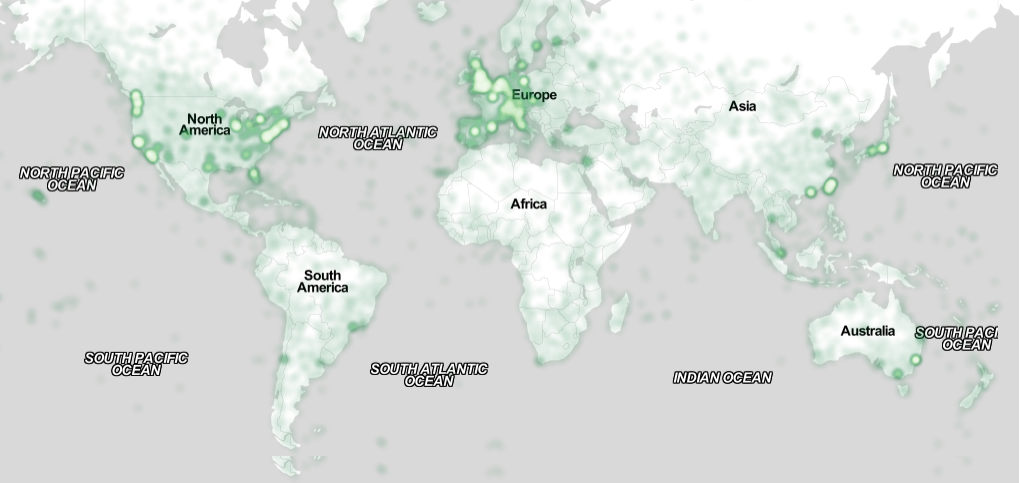
\includegraphics[width=\textwidth]{res/map}
\caption{A sample black and white graphic
that needs to span two columns of text.}
\end{figure*}


\begin{figure}

\includegraphics[height=1in, width=1in]{res/cats}
\caption{A sample black and white graphic that has
been resized with the \texttt{includegraphics} command.}
\end{figure}

\subsection{Theorem-like Constructs}

Other common constructs that may occur in your article are the forms
for logical constructs like theorems, axioms, corollaries and proofs.
ACM uses two types of these constructs:  theorem-like and
definition-like.

Here is a theorem:
\begin{theorem}
  Let $f$ be continuous on $[a,b]$.  If $G$ is
  an antiderivative for $f$ on $[a,b]$, then
  \begin{displaymath}
    \int^b_af(t)\,dt = G(b) - G(a).
  \end{displaymath}
\end{theorem}

Here is a definition:
\begin{definition}
  If $z$ is irrational, then by $e^z$ we mean the
  unique number that has
  logarithm $z$:
  \begin{displaymath}
    \log e^z = z.
  \end{displaymath}
\end{definition}

The pre-defined theorem-like constructs are \textbf{theorem},
\textbf{conjecture}, \textbf{proposition}, \textbf{lemma} and
\textbf{corollary}.  The pre-defined de\-fi\-ni\-ti\-on-like constructs are
\textbf{example} and \textbf{definition}.  You can add your own
constructs using the \textsl{amsthm} interface\footnote{\url{https://ctan.org/pkg/amsthm}}.  The
styles used in the \verb|\theoremstyle| command are \textbf{acmplain}
and \textbf{acmdefinition}.

Another construct is \textbf{proof}, for example,

\begin{proof}
  Suppose on the contrary there exists a real number $L$ such that
  \begin{displaymath}
    \lim_{x\rightarrow\infty} \frac{f(x)}{g(x)} = L.
  \end{displaymath}
  Then
  \begin{displaymath}
    l=\lim_{x\rightarrow c} f(x)
    = \lim_{x\rightarrow c}
    \left[ g{x} \cdot \frac{f(x)}{g(x)} \right ]
    = \lim_{x\rightarrow c} g(x) \cdot \lim_{x\rightarrow c}
    \frac{f(x)}{g(x)} = 0\cdot L = 0,
  \end{displaymath}
  which contradicts our assumption that $l\neq 0$.
\end{proof}

\section{Conclusions}
This paragraph will end the body of this sample document.
Remember that you might still have Acknowledgments or
Appendices; brief samples of these
follow.  There is still the Bibliography to deal with; and
we will make a disclaimer about that here: with the exception
of the reference to the \LaTeX\ book, the citations in
this paper are to articles which have nothing to
do with the present subject and are used as
examples only.
%\section{Conclusion}
The conclusion.

\printbibliography

\end{document}
